\chapter{Evaluación}
\label{Evaluación}

Este capítulo demuestra la validez de la solución construida. Describe primero el protocolo
experimental —qué se mide, cómo se mide y por qué el diseño permite atribuir las diferencias
observadas al método y no al montaje— y analiza después los resultados de los tres experimentos
realizados: la comparación principal entre las dos políticas, la curva de eficiencia en datos y la
medida de latencia de inferencia.

Se ha puesto especial cuidado en separar lo que los datos sostienen de lo que sugieren. Varias de
las conclusiones de este capítulo son deliberadamente más débiles de lo que las cifras brutas
invitarían a escribir, y en cada caso se explica por qué.


\section{Proceso de evaluación}

\subsection{Forma de evaluación}

\subsubsection{Métricas}

Se emplean dos métricas, ambas registradas automáticamente por el simulador:

\begin{description}
	\item[tasa de éxito]: proporción de episodios en los que la válvula supera media vuelta de
	apertura. Es la métrica principal.
	\item[tasa de movimiento de la articulación]: proporción de episodios en los que la válvula
	llega a moverse, con independencia de cuánto. Distingue el fallo por no completar el giro del
	fallo por no encontrar siquiera la válvula.
\end{description}

Se acompañan del ángulo final alcanzado por el volante, que permite ver la distribución de los
fallos en lugar de reducirlos a un contador.

\subsubsection{El banco es común a las dos políticas}

Las dos políticas se sirven como procesos independientes que implementan la misma interfaz de
comunicación con el simulador. El comando que lanza la evaluación es idéntico para ambas hasta el
último carácter: mismo entorno, mismo \textit{embodiment}, misma semilla y mismo presupuesto de
episodio. Lo único que cambia es qué proceso atiende la petición. Cualquier diferencia en la tasa de
éxito procede, por construcción, de la política.

\subsubsection{El diseño es emparejado}

Las condiciones iniciales de cada episodio —posición y orientación de la válvula— se generan a
partir de una semilla fija, de modo que la tirada $i$ de una política se enfrenta exactamente a la
misma escena que la tirada $i$ de la otra. Se ha verificado que las poses registradas coinciden
hasta el noveno decimal.

Esto convierte el experimento en un diseño de medidas emparejadas, y el contraste apropiado es la
\textbf{prueba exacta de McNemar} sobre los casos discordantes. Emplear una comparación de
proporciones independientes desaprovecharía la información del emparejamiento y sobreestimaría la
incertidumbre. Los intervalos de confianza de las tasas individuales se calculan por el método de
Wilson, que a diferencia del intervalo normal se mantiene dentro de $[0,1]$ con proporciones
próximas a los extremos, que es justo donde caen estos resultados.

\subsection{Casos de prueba}

\subsubsection{Ensayo previo de la cadena}

Pasada completa con veinticinco demostraciones de una sola disposición, con el único objetivo de
recorrer la cadena entera con datos reales y localizar dónde se rompe. Ambas políticas alcanzaron
diez éxitos de diez, lo que \textbf{no distingue nada}: sirve para afirmar que la cadena funciona,
no para comparar métodos.

\subsubsection{Comparación principal}

Doscientas tiradas por política, en dos bloques de cien con semillas distintas, sobre las políticas
entrenadas con las cien demostraciones definitivas.

\subsubsection{Curva de eficiencia en datos}

Reentrenamiento de ambos métodos sobre subconjuntos \textbf{estratificados y anidados} de
veinticinco y cincuenta demostraciones, y evaluación de las seis configuraciones resultantes sobre
las mismas cien condiciones iniciales. La estratificación es esencial: las primeras sesiones
grabadas se escoraron hacia la disposición difícil, de modo que tomar «las primeras veinticinco»
habría confundido \textit{menos datos} con \textit{más disposición difícil} y la curva habría caído
por el motivo equivocado.

\subsubsection{Latencia de inferencia}

Medida del tiempo de cálculo de cada bloque de acciones en lazo cerrado dentro del simulador, con
las observaciones reales y no con entradas sintéticas, y contraste contra el presupuesto que impone
el lazo de control.


\section{Análisis de resultados}

\subsection{Convergencia del entrenamiento}

\begin{figure}[htb]
\centering
  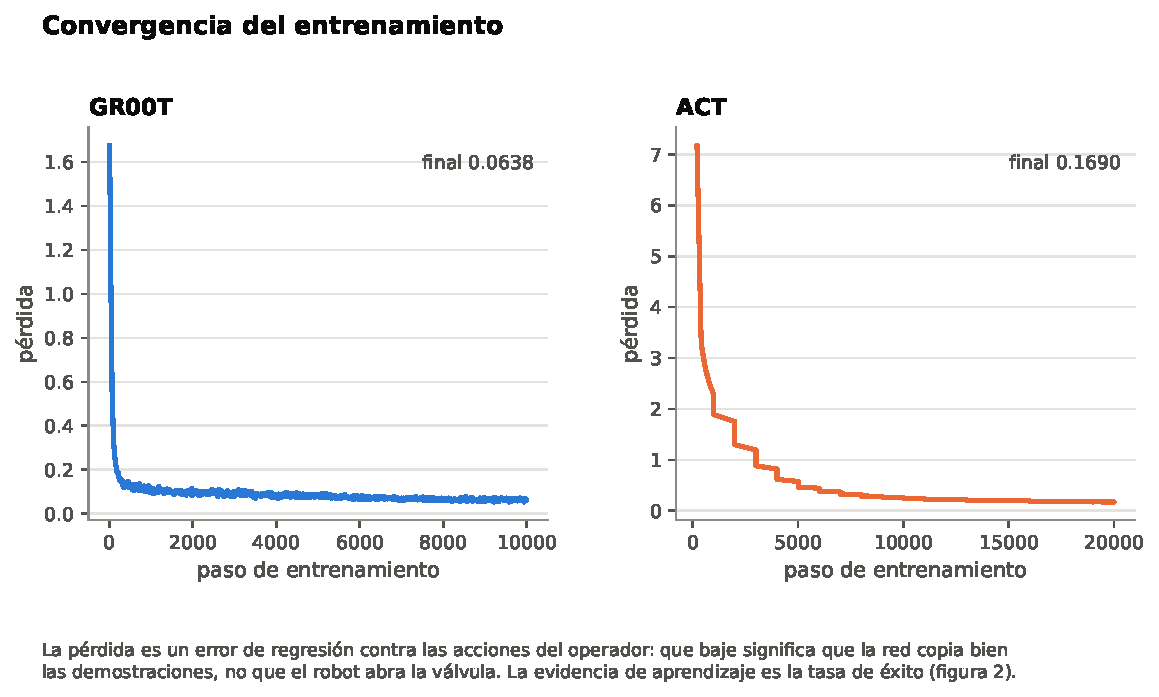
\includegraphics[width=\textwidth]{figuras/resultados/fig1_curvas_perdida.pdf}
  \caption[Convergencia del entrenamiento]{Convergencia del entrenamiento de ambos métodos, en
  paneles separados}
  \label{fig:perdida}
\end{figure}

Ambos entrenamientos convergen. Conviene subrayar, no obstante, que la pérdida en aprendizaje por
imitación es un error de regresión contra las acciones del operador: que baje significa que la red
copia bien las demostraciones, no que el robot abra la válvula. Una política puede exhibir una
pérdida excelente y una tasa de éxito nula si aprende la media de las demostraciones. La evidencia
de aprendizaje es la tasa de éxito en simulación; las curvas solo acreditan que la optimización
convergió. Las dos pérdidas, además, no son comparables entre sí, y por eso van en paneles
separados.

\subsection{Comparación principal}

\begin{table*}[ht]
	\centering
	\caption{Resultado sobre doscientas tiradas por política}
	\label{tab:resultado-principal}
	\makebox[\textwidth]{
		\begin{tabular}{|l|c|c|c|c|c|}
			\cline{1-6}
			Política & Tiradas & Éxito & IC 95\,\% & Movió la válvula & Ángulo medio \\ \hline
			GR00T N1.7 & 200 & \textbf{92\,\%} (185/200) & 88--95\,\% & 100\,\% & 177\textdegree \\
			ACT & 200 & \textbf{86\,\%} (172/200) & 81--90\,\% & 100\,\% & 173\textdegree \\ \hline
		\end{tabular}
	}
\end{table*}

\begin{figure}[htb]
\centering
  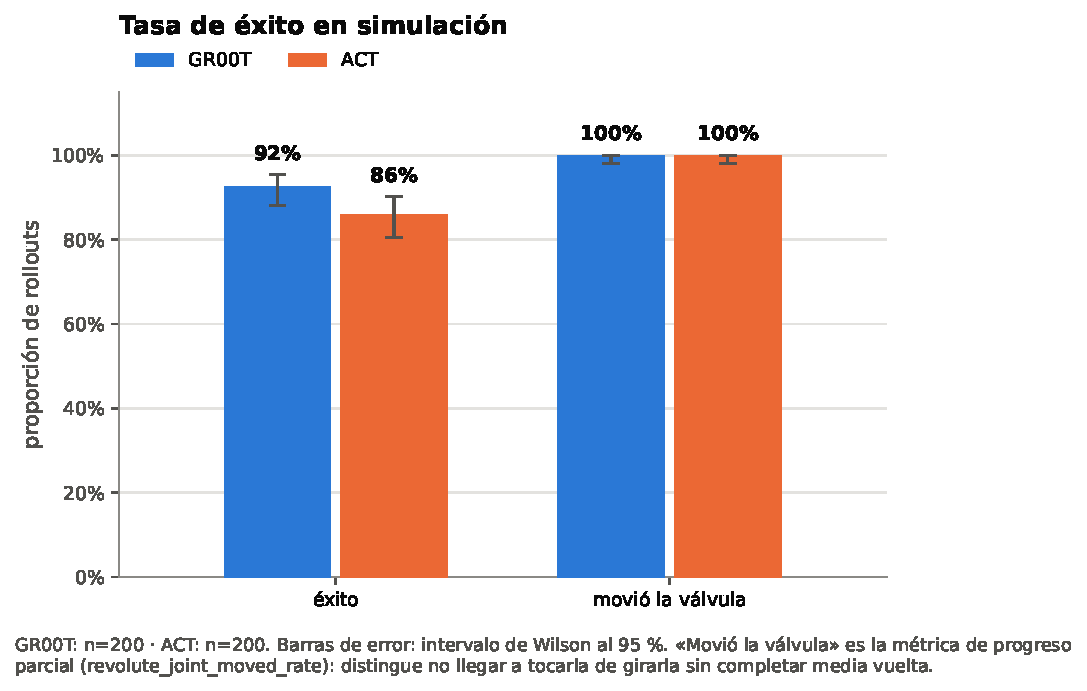
\includegraphics[width=\textwidth]{figuras/resultados/fig2_tasa_exito.pdf}
  \caption[Tasa de éxito de ambas políticas]{Tasa de éxito de ambas políticas con intervalos de
  confianza de Wilson al 95\,\%}
  \label{fig:tasa-exito}
\end{figure}

\subsubsection{El contraste emparejado}

De las doscientas tiradas, ciento sesenta las resuelven ambas políticas, veinticinco solo GR00T,
doce solo ACT y tres ninguna. La prueba exacta de McNemar sobre los treinta y siete casos
discordantes arroja $p = 0{,}047$.

\textbf{Ese valor cruza el umbral del 5\,\% por un solo episodio y es frágil.} Un reparto de
veinticuatro contra trece daría $p = 0{,}099$, y de veinticinco contra trece, $p = 0{,}073$. La
afirmación que los datos sostienen es que \textit{GR00T va consistentemente por delante en los dos
bloques y la diferencia se aproxima a la significación estadística}; afirmar que GR00T es
significativamente mejor que ACT sería sobreinterpretar el resultado.

\subsubsection{Dónde vive la diferencia}

\begin{figure}[htb]
\centering
  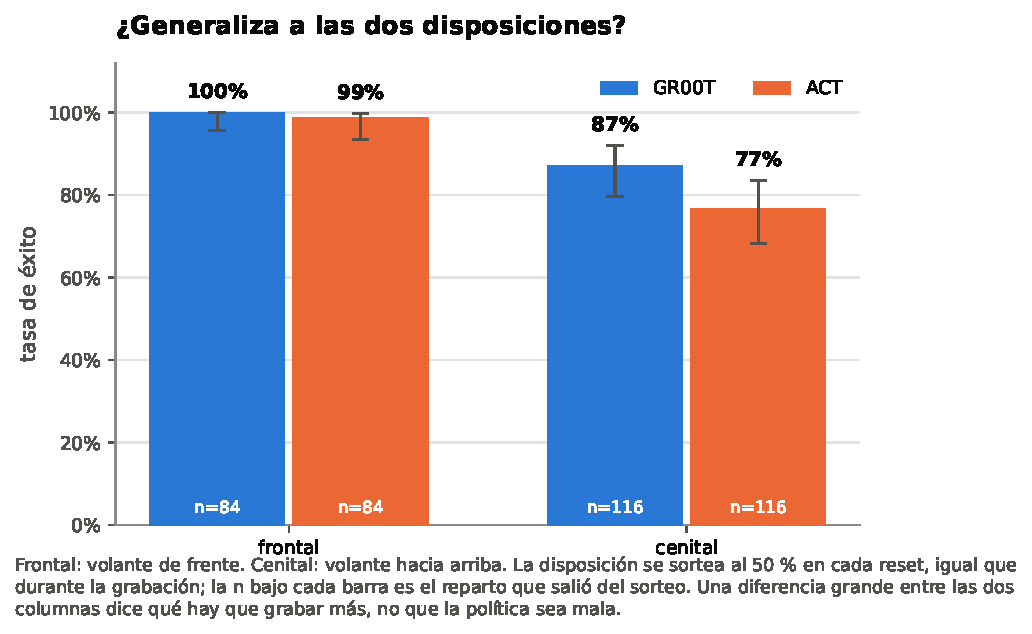
\includegraphics[width=\textwidth]{figuras/resultados/fig4_exito_por_disposicion.pdf}
  \caption[Tasa de éxito por disposición de la válvula]{Tasa de éxito de cada política separada por
  disposición de la válvula}
  \label{fig:por-disposicion}
\end{figure}

Lo que sí resulta significativo, y con mucho margen, es el efecto de la disposición: ambas políticas
son claramente peores con la válvula en posición cenital. Y toda la diferencia entre métodos vive
ahí: treinta y seis de los treinta y siete casos discordantes son cenitales, mientras que la
disposición frontal está saturada para las dos. La afirmación defendible es, por tanto, que
\textit{GR00T aguanta algo mejor la disposición difícil}, no que sea mejor en general.

\subsection{Distribución de los fallos}

\begin{figure}[htb]
\centering
  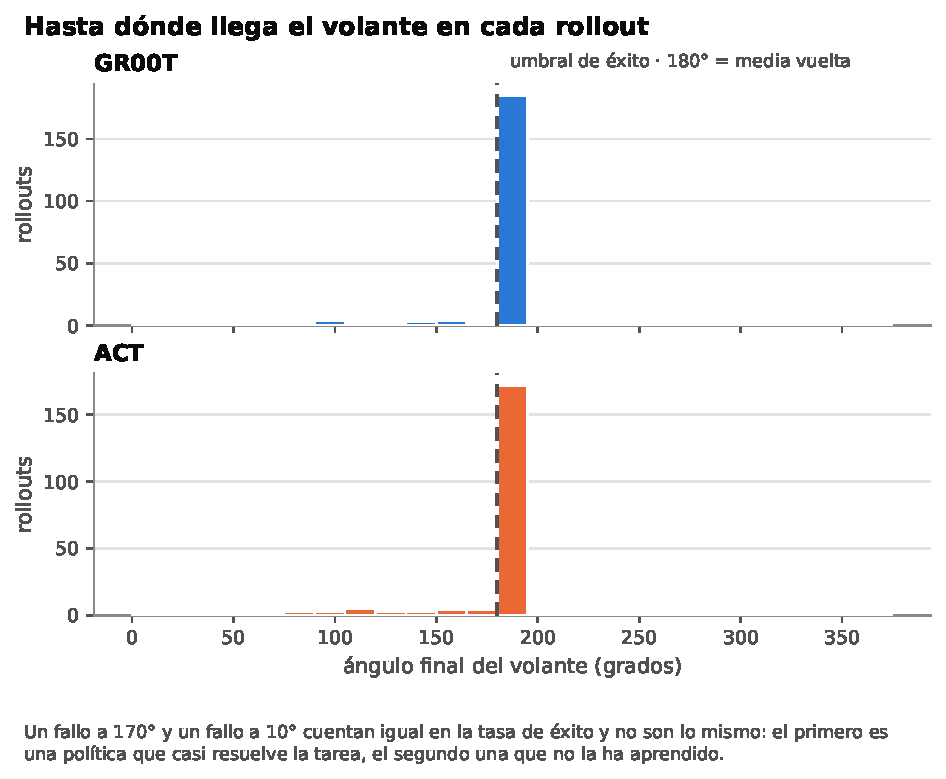
\includegraphics[width=\textwidth]{figuras/resultados/fig3_distribucion_angulo.pdf}
  \caption[Distribución del ángulo final alcanzado]{Distribución del ángulo final alcanzado por el
  volante, con el umbral de éxito marcado}
  \label{fig:angulos}
\end{figure}

La tasa de movimiento de la articulación resulta del 100\,\% para ambas políticas en las
cuatrocientas tiradas, de modo que no discrimina en esta comparación. Pero es en sí misma un
resultado: no hay ni un solo episodio en el que el robot no llegue a alcanzar la válvula. Todos los
fallos son de \textit{no completar media vuelta}, nunca de \textit{no encontrarla}.

\subsection{Eficiencia en datos}

\begin{figure}[htb]
\centering
  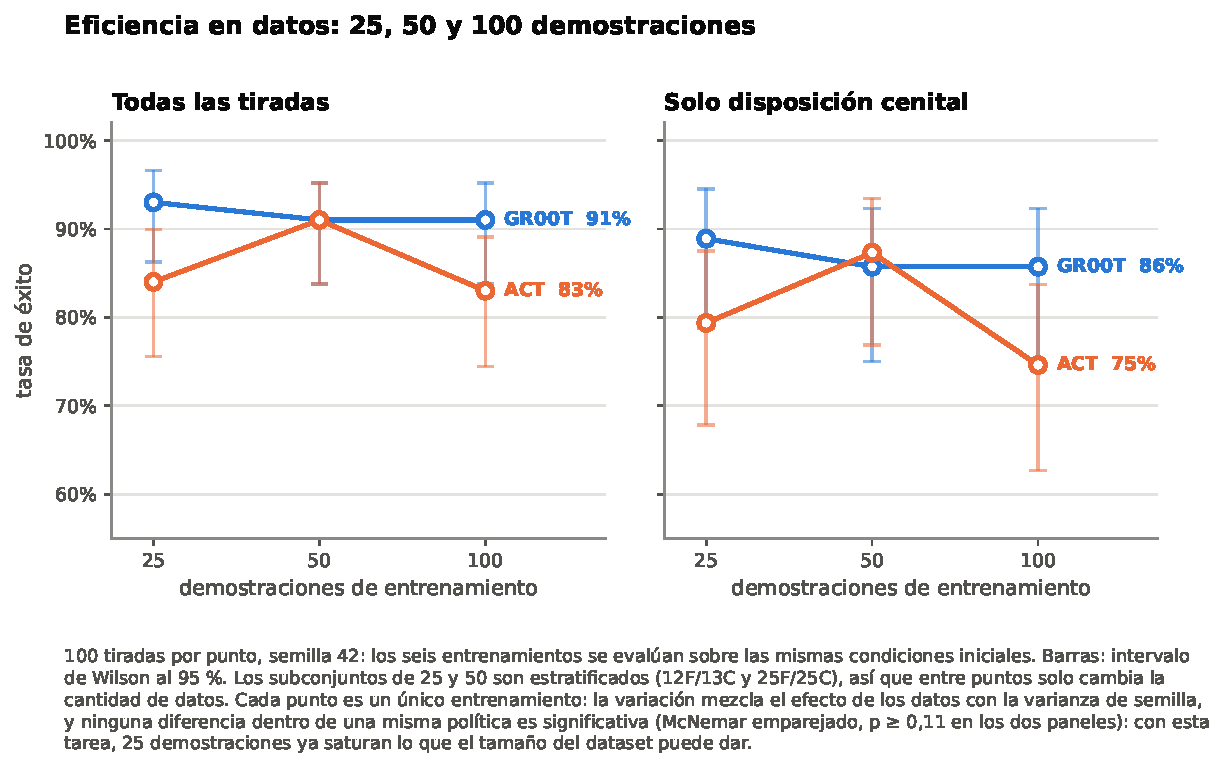
\includegraphics[width=\textwidth]{figuras/resultados/fig8_curva_eficiencia.pdf}
  \caption[Curva de eficiencia en datos]{Tasa de éxito frente al número de demostraciones de
  entrenamiento, en el total de las tiradas y restringida a la disposición cenital}
  \label{fig:eficiencia}
\end{figure}

La hipótesis que justifica el empleo de un modelo fundacional era que GR00T se despegara con pocas
demostraciones y ACT necesitara más. \textbf{No se observa.} Ninguna diferencia dentro de una misma
política resulta significativa. El resultado es negativo y es el más útil del experimento: el
margen de fallo restante \textbf{no es un problema de cantidad de datos}, sino de su composición.

Debe leerse con una cautela que se hace explícita: cada punto de la curva corresponde a un único
entrenamiento, de modo que la variación entre puntos mezcla el efecto de los datos con la varianza
de semilla del propio entrenamiento.

\subsection{Latencia de inferencia}

\begin{figure}[htb]
\centering
  
\includegraphics[width=\textwidth]{figuras/resultados/fig9_latencia.pdf}
  \caption[Coste de inferencia frente al presupuesto de tiempo real]{Coste de inferencia de cada
  política frente al presupuesto que impone el lazo de control}
  \label{fig:latencia}
\end{figure}

La diferencia de sesenta y un veces en número de parámetros se traduce en diez veces en latencia, y
aun así ambas políticas caben holgadamente dentro del presupuesto. La latencia no es, en esta tarea
y sobre este equipamiento, un argumento en contra del modelo fundacional.

\subsection{Amenazas a la validez}

Discusión honesta de los límites del experimento: una sola tarea, una sola semilla de entrenamiento
por configuración, ausencia de validación sobre robot físico, y el hecho de que las demostraciones
terminan justo al cruzar el umbral de éxito, lo que hace que parte de los fallos sean casi-éxitos
por construcción del protocolo de captura.
